\section{Model}
\label{sec:model}

\subsection{Notation and Composition}
\label{sec:notation}

PBM operates on sRGB display values in $[0,1]$; no linearization, transfer function, or color-space conversion is applied. The model is the composition of a mixing core and a repair layer,
\begin{equation}
\mathbf{o}=\clamp\bigl(\mathbf{C}+\mathbf{d},\,0,\,1\bigr),\qquad
\mathbf{C}=\operatorname{Core}(\cb,\ct,\alpha),\qquad
\mathbf{d}=\operatorname{Repair}(\cb,\ct,\alpha,\mathbf{C}),
\label{eq:composition}
\end{equation}
where $\cb$ is the base color, $\ct$ the tint, and $\alpha=\clamp(A,0,1)$ the tint share: $\alpha=0$ returns the base and $\alpha=1$ the tint.

\begin{figure}[t]
\centering
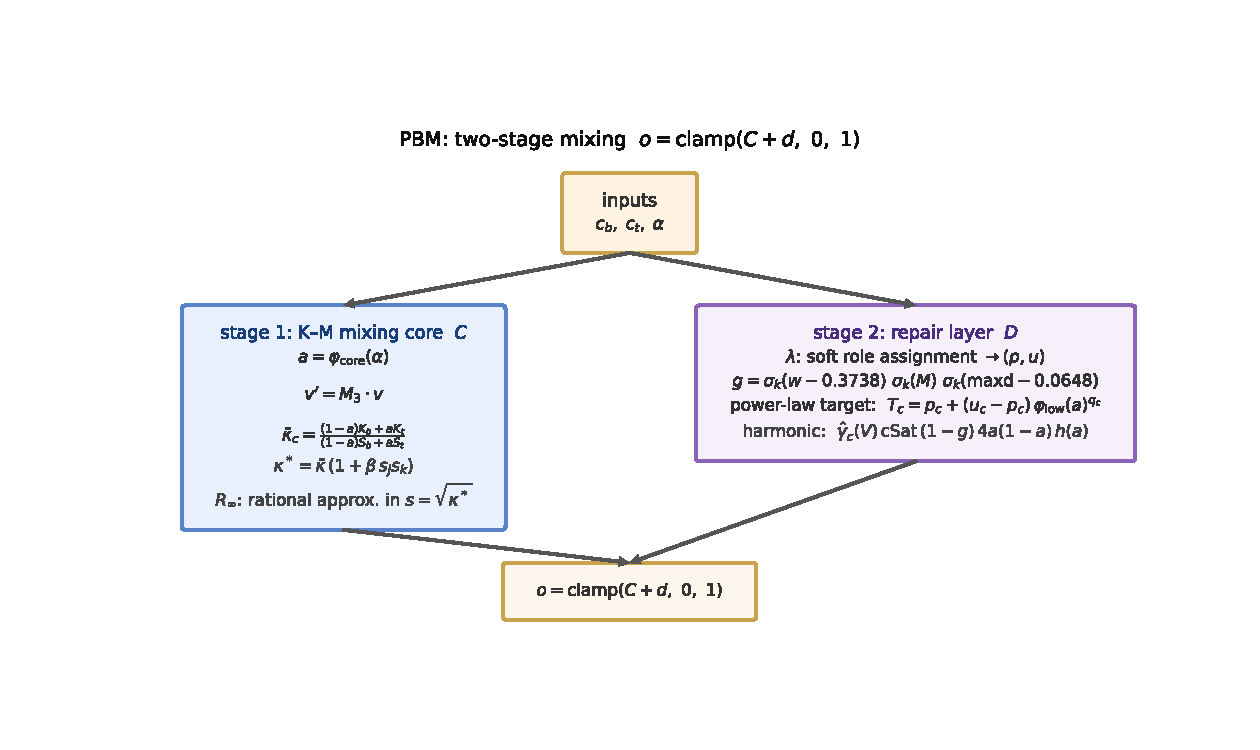
\includegraphics[width=0.82\linewidth]{fig2-architecture.pdf}
\caption{PBM data flow. Both inputs feed the K--M mixing core ($C$). The repair layer assigns the pigment and bright-end roles ($\lambda$), evaluates the per-channel power-law target ($T$) gated by $g$, and adds the harmonic correction ($\hat{\gamma}$). The correction $\mathbf{d}$ is added to the core output and clamped.}
\label{fig:architecture}
\end{figure}

The repair layer is asymmetric in the roles of its two arguments, whereas the core is symmetric. A soft role assignment blends the two role orderings so that the complete model is exchange-symmetric,
\begin{equation}
F(\cb,\ct,\alpha)\equiv F(\ct,\cb,1-\alpha),
\label{eq:symmetry}
\end{equation}
up to floating-point rounding.

We write $\vp$ for the pigment endpoint and $\vu$ for the bright endpoint, as selected by the role assignment (\cref{sec:role}): the input with the smaller maximum channel plays the pigment. From $\vp$ we define
\begin{equation}
M=\max(\vp),\qquad m=\min(\vp),\qquad \mathrm{maxd}=M-m,\qquad
w=\max\bigl(\min(\vp),\min(\vu)\bigr).
\label{eq:notation}
\end{equation}
The soft step with slope $k$ is $\sigmak(x)=\clamp(kx,0,1)$, and $\ssf(x;a,b)$ is the $C^{1}$ smoothstep on $[a,b]$.

\subsection{The Structural Limitation of Display-Value K/S Mixing}
\label{sec:defect}

The core mixes in display-value space using analytic defaults for absorption and scattering,
\begin{equation}
K(v)=\tfrac12(1-v)^{2},\qquad S(v)=\max(v,\varepsilon),\qquad \varepsilon=0.00157634.
\label{eq:ks-default}
\end{equation}
For a white input, $v=1$, hence $K=0$ and $S=1$, whereas a deep pigment has $S$ in the range $0.05$--$0.35$. At any $\alpha$, the scattering of white dominates the denominator of the concentration-weighted ratio, and the per-channel $\kappa$ values collapse toward each other.

As a single-channel illustration, ignore the cross-channel matrix and the mutual-absorption correction and consider the red channel of the deep blue $\#0D1B44=(0.051,0.106,0.267)$ mixed with white at $\alpha=0.5$:
\begin{equation}
\bar{\kappa}_{R}=
\frac{0.5\,K(0.051)+0.5\,K(1)}{0.5\,S(0.051)+0.5\,S(1)}
=\frac{0.5\times0.451}{0.5\times0.051+0.5\times1}=0.429,
\label{eq:defect}
\end{equation}
which gives $\Rinf\approx0.41$. The Mixbox reference reads $0.28$ for this channel. The absorbing channel is washed out. Conversely, the blue channel reads $0.89$ in the reference against $0.53$ in the single-channel computation; it is under-lightened. This imbalance is structural: the $S=1$ of white dominates the mixture denominator for every $\alpha$, and the weighted $K$ and $S$ are constrained by the same weights, so rescaling $K/S$ at the mixing stage cannot restore the absorbed channel. Raw display-value K--M superposition measures a mean $\Delta E_{00}$ of 10.30 on the dark-plus-white suite (\cref{tab:insample}).

\subsection{Stage 1: The K--M Mixing Core}
\label{sec:core}

Both inputs are transformed by a cross-channel matrix $\Mthree$ with row sums equal to one,
\begin{equation}
\mathbf{v}'=\Mthree\mathbf{v},\qquad
\Mthree=
\begin{pmatrix}
0.74523981 & 0.30403013 & -0.04926994\\
0 & 0.74093256 & 0.25906744\\
0 & 0 & 1
\end{pmatrix}.
\label{eq:m3}
\end{equation}
Absorption and scattering are evaluated with the analytic defaults of \cref{eq:ks-default}. The mixing ratio in each channel follows Duncan's concentration structure, clamped to $[10^{-6},10^{4}]$:
\begin{equation}
\bar{\kappa}_{c}=
\frac{(1-a)\,K(v'_{b,c})+a\,K(v'_{t,c})}
     {(1-a)\,S(v'_{b,c})+a\,S(v'_{t,c})},
\label{eq:kappa}
\end{equation}
where $a=\varphi_{\mathrm{core}}(\alpha)$ is the progress after endpoint compression.

A per-channel mutual-absorption correction uses the other two channels $\{j,k\}$:
\begin{equation}
s'_{c}=\frac{\sqrt{\bar{\kappa}_{c}}}{1+\sqrt{\bar{\kappa}_{c}}},\qquad
\kstar_{c}=\bar{\kappa}_{c}\bigl(1+\beta_{c}\,s'_{j}\,s'_{k}\bigr),\qquad
\beta=(-0.69372345,\,-0.48397409,\,-0.24977842).
\label{eq:beta}
\end{equation}
Because $s'\in[0,1)$ and $\beta_{c}<0$, the correction reduces $\kappa$ when the other channels are bright.

The reflectance is evaluated with a rational approximation in $s=\sqrt{\kstar}$,
\begin{equation}
\Rinf\approx\frac{1}{1+s\bigl(a_{1}+s(a_{2}+s\,a_{3})\bigr)},\qquad
(a_{1},a_{2},a_{3})=\Bigl(\sqrt{2},\,1,\,\tfrac{1}{2\sqrt{2}}\Bigr),
\label{eq:rational}
\end{equation}
which matches the first four Taylor coefficients of $\Rinf$ at $s=0$. Over the clamped range $\kstar\in[10^{-6},10^{4}]$, the maximum absolute error of \cref{eq:rational} is $8.1\times10^{-3}$ (at $\kstar\approx8.1$); for $\kstar\le1$ it is $2.5\times10^{-3}$. The output is mapped back and clamped:
\begin{equation}
\mathbf{C}=\clamp\bigl(\Mthree^{-1}\,\Rinf(\boldsymbol{\kstar}),\,0,\,1\bigr).
\label{eq:core-output}
\end{equation}

\paragraph{Dynamic progress.}
The reference converges faster than display-value $\kappa$ mixing as $\alpha\to1$. Inverting the reference at $\alpha=0.99$ indicates that the power-law target would require an equivalent progress of about $10^{-3}$ (\cref{sec:inversion}), i.e.\ that 99\% of the blend behaves like 99.9\%. We encode this with a symmetric endpoint-compression map applied to the core's mixing ratio,
\begin{equation}
\varphi_{\mathrm{low}}(x)=
\begin{cases}
x, & x\ge w_{\varphi},\\[2pt]
\bigl(1-\ssf(x;0,w_{\varphi})\bigr)x^{p_{\varphi}}+\ssf(x;0,w_{\varphi})\,x, & x<w_{\varphi},
\end{cases}
\label{eq:philow}
\end{equation}
\begin{equation}
\varphi_{\mathrm{core}}(x)=
\begin{cases}
\varphi_{\mathrm{low}}(x), & x<0.5,\\
1-\varphi_{\mathrm{low}}(1-x), & x\ge0.5,
\end{cases}
\label{eq:phicore}
\end{equation}
with $p_{\varphi}=1.96522814$ and $w_{\varphi}=0.08$. The map is $C^{1}$ and antisymmetric about $x=0.5$, so the core remains exchange-symmetric; $\varphi_{\mathrm{low}}(x)=x$ for $x\ge w_{\varphi}$, so only the tails are affected.

\subsection{Stage 2: The Repair Layer}
\label{sec:repair}

The repair layer computes a correction $\mathbf{d}$ to the core output. It consists of a role assignment, a gate, a per-channel power-law target, and an additive harmonic correction.

\paragraph{Soft role assignment.}
\label{sec:role}
The pigment endpoint is the input with the smaller maximum channel. A hard argmin would switch discontinuously when $\max(\cb)=\max(\ct)$, so we use a soft membership
\begin{equation}
\lambda=\ssf\!\left(\frac{\max(\ct)-\max(\cb)+E_{W}}{2E_{W}};\,0,\,1\right),
\qquad E_{W}=0.08.
\label{eq:lambda}
\end{equation}
$\lambda=1$ selects $(\vp,\vu,a)=(\cb,\ct,\alpha)$; $\lambda=0$ selects $(\ct,\cb,1-\alpha)$; inside the tie band $|\max(\ct)-\max(\cb)|<E_{W}$ the two branches are blended,
\begin{equation}
\mathbf{d}=\lambda\,D(\cb,\ct,\alpha)+(1-\lambda)\,D(\ct,\cb,1-\alpha).
\label{eq:dblend}
\end{equation}
Outside the band, $\lambda$ is exactly $0$ or $1$ and the layer reduces to one evaluation of $D$. For uniformly sampled sRGB pairs, the band contains approximately $26\%$ of pairs (measured $26.6\%$ on the T3 draw with seed 20260808 and $26.2\%$ on $2\times10^{5}$ uniform pairs); the branch is therefore skipped for about three quarters of random inputs. The role signal is the maximum channel; a luminance signal was also considered but changed the role decision for a non-negligible fraction of random pairs and was not adopted.

\paragraph{Dark-plus-light gate.}
The power-law target is applied only in the dark-pigment/light-end region. The gate is a product of three soft steps with the shared slope $k=11.0163945$:
\begin{equation}
g=\sigmak(w-0.37375181)\cdot\sigmak(M)\cdot\sigmak(\mathrm{maxd}-0.06479933).
\label{eq:gate}
\end{equation}
The first factor opens when the brighter endpoint is close to achromatic-bright ($w$ large); the second reduces the gate for near-black pigments ($M\lesssim1/k\approx0.09$); the third requires a minimum chroma range. Each transition has width $1/k\approx0.091$, so the gate introduces no hard cutoff. For light or nearly achromatic pigments, $g=0$ and the core output is used directly.

\paragraph{Power-law target.}
Within the gate region, the target follows a per-channel power law from the pigment toward the bright end:
\begin{equation}
T_{c}=p_{c}+(u_{c}-p_{c})\,\varphi_{\mathrm{low}}(a)^{q_{c}}.
\label{eq:target}
\end{equation}
The exponent $q_{c}$ controls how quickly channel $c$ brightens and is composed of four terms.

\emph{(a) Soft-step staircase.} Inverting the reference on anchored colors (\cref{sec:inversion}) shows that the required exponent decreases with the channel value $v$: dark segments hold absorption (high $q$), bright segments advance quickly (low $q$). The structure is represented by two steps,
\begin{equation}
q^{f}(v)=c_{1}^{f}+(c_{2}^{f}-c_{1}^{f})\,\sigmak(v-t_{1})+(c_{3}-c_{2}^{f})\,\sigmak(v-t_{2}),
\qquad f\in\{B,G\},
\label{eq:staircase}
\end{equation}
with $t_{1}=0.04350222$, $t_{2}=0.26436295$, and the coefficients in \cref{tab:softstep}. The red family is neutral, $q^{R}\equiv1$; its channel-dependent behavior is carried by the directional responses in (d).

\begin{table}[t]
\centering
\small
\caption{Soft-step coefficients of the brightening exponent (\cref{eq:staircase}).}
\label{tab:softstep}
\begin{tabular}{lcccc}
\toprule
Family & $c_{1}$ (dark) & $c_{2}$ (mid) & $c_{3}$ (bright) & Step positions / slope \\
\midrule
$B$ (blue, $B$ maximal) & 0.91483121 & 0.32538955 & 0.18785981 & $t_{1}=0.04350222$, $t_{2}=0.26436295$ \\
$G$ (green, $G$ maximal) & 0.57387051 & 0.596528 & 0.18785981 & $k=11.0163945$ (shared) \\
$R$ (red) & --- & --- & --- & $q^{R}\equiv1$ \\
\bottomrule
\end{tabular}
\end{table}

\emph{(b) Family soft mixing.} The family weights are pairwise dominance comparisons on the pigment channels,
\begin{equation}
g_{R}=\tfrac12\,\sigma_{8}(v_{R}-v_{G})+\tfrac12\,\sigma_{8}(v_{R}-v_{B}),
\qquad g_{G},,g_{B}\ \text{analogously},
\label{eq:family-weights}
\end{equation}
where $\sigma_{8}(x)=\clamp(8x,0,1)$. The base exponent is
\begin{equation}
q_{c}^{\mathrm{base}}=\frac{g_{B}q_{c}^{B}+g_{G}q_{c}^{G}+g_{R}q_{c}^{R}}{g_{R}+g_{G}+g_{B}}.
\label{eq:qbase}
\end{equation}
When $g_{R}+g_{G}+g_{B}<10^{-6}$, the base reduces to the equal-weight mean, which covers near-gray pigments.

\emph{(c) Channel residuals.} For near-zero channels, the reference curves depend on the channel rather than on the pigment. The residual is a shared amplitude times a smooth envelope,
\begin{equation}
q_{c}\mathrel{+}=\mathrm{RES}_{c}\,e(v_{c}),\qquad
e(v)=
\begin{cases}
A\bigl(1-v/W\bigr)^{2}, & v<W,\\
0, & v\ge W,
\end{cases}
\label{eq:residual}
\end{equation}
with $A=0.83421324$, $W=0.14196781$, and $\mathrm{RES}=(0,\,-0.24164942,\,-0.24164942)$; the red residual is zero. Unlike a piecewise-linear envelope, \cref{eq:residual} is $C^{1}$ at $v=W$ and needs three constants instead of eight.

\emph{(d) Channel coupling and directional responses.} Colors with two high channels brighten more slowly, and each family carries a linear directional response in the pigment channels:
\begin{equation}
q_{c}\mathrel{+}=0.42818849\,\sigma_{4.13539205}\Bigl(\max_{i\ne c}v_{i}\Bigr),
\label{eq:coupling}
\end{equation}
\begin{equation}
q_{c}\mathrel{+}=g_{R}\,g^{\mathrm{RTH}}\,\delta^{R}_{c}+g_{B}\,\delta^{B}_{c}+g_{G}\,\delta^{G}_{c},
\qquad
g^{\mathrm{RTH}}=\sigma_{8}(v_{R}-0.21929798),
\label{eq:directional}
\end{equation}
with
\begin{align}
\delta^{R}&=\bigl[-0.28030789-0.31011215\,v_{R},\nonumber\\
&\qquad 0.33194666-1.19791733\,v_{G},\; -0.45218018+1.71390058\,v_{G}\bigr],\nonumber\\
\delta^{B}&=\bigl[0.40713961,\; -0.08390816+0.76274462\,v_{G},\; 0\bigr],\label{eq:deltas}\\
\delta^{G}&=\bigl[-0.2367074+0.72220875\,v_{R},\; 0,\; -0.30067864+1.03098891\,v_{G}\bigr].\nonumber
\end{align}
The range gate $g^{\mathrm{RTH}}$ is necessary: the linear expressions change sign below $v_{R}=0.21929798$. For the two near-black reds $\#280501$ and $\#250903$ over $\alpha\in[0.1,0.9]$, disabling the gate raises the mean $\Delta E_{00}$ from 2.80 to 15.76 (maximum from 4.14 to 19.04).

\paragraph{Harmonic correction.}
Inverting the reference on complementary pairs (\cref{sec:inversion}) reveals a residual concentrated in the middle of the mixing range with the shape $4a(1-a)$ and an amplitude that varies smoothly with the input colors. The correction is a linear model over a ratio-based feature template, attenuated at both endpoints:
\begin{equation}
d_{c}\mathrel{+}=\hat{\gamma}_{c}(\vp,\vu)\;\mathrm{cSat}(\vp,\vu)\;(1-g)\;4a(1-a)\;h(a),
\label{eq:harmonic}
\end{equation}
where
\begin{equation}
\begin{aligned}
h(a)&=\sigma_{14}(0.845-a),\\
\mathrm{cSat}(\vp,\vu)&=\ssf\bigl(\max(\vp)-\min(\vp);0.02,0.15\bigr)\\
&\qquad\cdot\ssf\bigl(\max(\vu)-\min(\vu);0.08,0.30\bigr).
\end{aligned}
\label{eq:csat}
\end{equation}
The factor $(1-g)$ excludes the dark-plus-light region. The chroma attenuation $\mathrm{cSat}$ drives the correction to zero when either endpoint approaches the achromatic axis. This attenuation is important for continuity: the ratio features have large gradients near zero chroma, and without $\mathrm{cSat}$ the maximum single-step output change under an 8-bit input perturbation rises from 1.39 to 2.53 $\Delta E_{00}$ (\cref{sec:continuity}).

The amplitude is a linear function of a seventeen-feature template $V$ computed once per pair,
\begin{equation}
\hat{\gamma}_{c}(\vp,\vu)=w_{0}^{c}+\sum_{j}w_{j}^{c}\,V_{j},
\label{eq:gamma}
\end{equation}
with $17$ coefficients per channel ($51$ in total), fitted by least squares on a corpus of complementary-family and random measurements (\cref{sec:estimation}). Every feature is a polynomial, a ratio of channel differences, or a clamped linear form: the template contains no trigonometric function, so the harmonic correction costs only multiplications, additions, and one division per ratio. The template is defined in \cref{tab:features}; the coefficients are listed in \cref{app:coeff}. Unlike a learned latent representation, the template is hand-designed from the inversion measurements, and no data are stored at runtime.

\begin{table}[t]
\centering
\scriptsize
\setlength{\tabcolsep}{3pt}
\caption{The harmonic feature template (seventeen features including the intercept, used by all three channels). All features are computed once per pair from the pigment endpoint $\vp$ and the bright endpoint $\vu$.}
\label{tab:features}
\begin{tabular}{ll}
\toprule
Feature & Definition \\
\midrule
intercept & $1$ \\
\texttt{lum} & $0.2126\,p_{R}+0.7152\,p_{G}+0.0722\,p_{B}$ \\
\texttt{lumU} & $0.2126\,u_{R}+0.7152\,u_{G}+0.0722\,u_{B}$ \\
\texttt{pm}, \texttt{pn} & $\max(\vp)$, $\min(\vp)$ \\
\texttt{Mmn} & $\max(\vp)\cdot\min(\vp)$ \\
\texttt{span} & $(\max(\vp)-\min(\vp))(\max(\vu)-\min(\vu))$ \\
\texttt{op} & $1-\tfrac12\bigl[(\max(\vp)-\min(\vp))+(\max(\vu)-\min(\vu))\bigr]$ \\
\texttt{u2} & $u_{B}$ \\
\texttt{dcAbs} & $|u_{R}-p_{R}|$ \\
\texttt{wUcP} & $(u_{R}-u_{B})(p_{B}-p_{R})$ \\
\texttt{dg}, \texttt{ur} & $d_{g}=(p_{G}-p_{B})/\max(M-m,\epsilon)$,\quad $u_{r}=(u_{R}-u_{B})/\max(u_{\max}-u_{\min},\epsilon)$ \\
\texttt{drur}, \texttt{dgug} & $d_{r}u_{r}$, $d_{g}u_{g}$, with $d_{r}=(p_{R}-p_{B})/\cdots$ and $u_{g}=(u_{G}-u_{B})/\cdots$ \\
\texttt{dcmucm} & $d_{cm}u_{cm}$, with $d_{cm}=(p_{R}-p_{G})/\cdots$ and $u_{cm}=(u_{R}-u_{G})/\cdots$ \\
\texttt{gRu} & $\tfrac12\sigma_{8}(u_{R}-u_{G})+\tfrac12\sigma_{8}(u_{R}-u_{B})$ \\
\bottomrule
\end{tabular}
\end{table}

\subsection{Algorithm and Boundary Behavior}
\label{sec:algorithm}

The complete procedure is given in \cref{alg:pbm}. The endpoint-copy step makes $\alpha=0$ and $\alpha=1$ exact by construction. All remaining operations are compositions of continuous functions---clamps, powers, smoothsteps, and linear forms---so the model is continuous; no branch changes the value of an output discontinuously. \Cref{tab:boundary} summarizes the boundary properties and the measured values.

Here $\operatorname{Core}$ denotes the composition of \cref{eq:phicore,eq:m3,eq:kappa,eq:beta,eq:core-output}, and $D$ denotes the repair branch of \cref{eq:gate,eq:target,eq:harmonic}.

\begin{algorithm}[t]
\caption{PBM mixing.}
\label{alg:pbm}
\KwIn{base $\cb$, tint $\ct$ (sRGB display values in $[0,1]$), ratio $A$}
\KwOut{mixed color $\mathbf{o}$}
$\alpha\gets\clamp(A,0,1)$\;
\If{$\alpha=0$}{\Return{$\cb$}}
\If{$\alpha=1$}{\Return{$\ct$}}
$\mathbf{C}\gets\operatorname{Core}(\cb,\ct,\alpha)$\;
$t_{e}\gets\clamp\bigl((\max(\ct)-\max(\cb)+E_{W})/(2E_{W}),0,1\bigr)$\;
\uIf{$t_{e}\le0$}{$\mathbf{d}\gets D(\ct,\cb,1-\alpha,\mathbf{C})$}
\uElseIf{$t_{e}\ge1$}{$\mathbf{d}\gets D(\cb,\ct,\alpha,\mathbf{C})$}
\Else{$\lambda\gets\ssf(t_{e})$;\; $\mathbf{d}\gets\lambda D(\cb,\ct,\alpha,\mathbf{C})+(1-\lambda)D(\ct,\cb,1-\alpha,\mathbf{C})$}
\Return{$\clamp(\mathbf{C}+\mathbf{d},0,1)$}\;
\end{algorithm}

\begin{table}[t]
\centering
\small
\caption{Boundary behavior of PBM.}
\label{tab:boundary}
\begin{tabular}{p{0.28\linewidth}p{0.64\linewidth}}
\toprule
Property & Guarantee \\
\midrule
$\alpha=0,1$ & returns the inputs exactly (T4 maximum channel error 0.00000). \\
Outside the gate & $g=0$: core output plus the harmonic correction; inside: power-law target plus harmonic correction; the transition is continuous. \\
Continuity & composition of continuous functions; measured maximum single-step $\Delta E_{00}$ of 1.388 under an 8-bit perturbation, with zero exceedances of 1.53. \\
Exchange symmetry & $F(\cb,\ct,\alpha)\equiv F(\ct,\cb,1-\alpha)$; maximum observed RGB difference $6.7\times10^{-16}$ over 5000 random pairs (seed 20260808). \\
\bottomrule
\end{tabular}
\end{table}

\paragraph{Complexity and implementation.}
The model performs a fixed number of arithmetic operations: two matrix-vector products for the inputs, one for the output, six square roots, up to five powers, and no trigonometric or logarithmic evaluation. It has no loops over data, no tables, and no iteration; its time and space complexity is $O(1)$. A reference implementation is available in four languages (JavaScript, Python, Java, and C++) with identical constants; a cross-language test over 2000 random pairs measures a maximum RGB channel difference of $5\times10^{-10}$, which is consistent with the nine-decimal serialization used by the test and with library-level differences in the elementary functions.

The constants of the model are frozen in the implementation. Changing them requires re-running the estimation and the cross-language consistency test; the four ports are kept identical at the level of numeric literals.
